\documentclass[12pt]{report}
\usepackage[margin=1in]{geometry}
\usepackage{multicol}
\usepackage{caption}
\usepackage{subcaption}
\usepackage{graphicx}
\usepackage{float}
\usepackage{epstopdf}
\usepackage{setspace}
\usepackage{abstract}
%\usepackage{grffile}
\usepackage{pdfpages}
\usepackage{lscape}
\usepackage{authblk}
\usepackage{hyperref}
\usepackage{longtable}


%Graphics Path
\graphicspath{{./MCINTOSH_Images/}{./WILEY_Images/}{./KIRBY_Images/}{./WESLEY_Images/}{./IANNUCCI_Images/}{./BLUM_Images/}{./REGAN_Images/}{./PAUL_Images/}}

\usepackage{fancyhdr}
	\pagestyle{fancy}
	\fancyhead[L]{\today}
	\fancyfoot{}
	\fancyhead[C]{OCE 496 Section 2}
	\fancyhead[R]{\thepage}


\title{\vspace{-5mm}
	\fontsize{20pt}{10pt}\selectfont
	Embedded Wireless Sensor Design for Long Term Structural Health Monitoring
}
		
\author[2]{Christopher Bessin}	
\author[1]{Patrick Blum}
\author[1]{Matthew P. Iannucci}
\author[1]{Jordan T. Kirby}
\author[1]{Zachary McIntosh}
\author[2]{Elizabeth L. Paul}
\author[1]{Michael A. Regan}
\author[2]{Justin W. Skenyon}
\author[1]{Charles J. Wesley}
\author[1]{Samuel D. Wiley}

\affil[1]{Finite Element Modelling}
\affil[2]{Instrumentation Development}
\date{\normalsize\vspace{-3mm}\today}



\begin{document}
\maketitle

%Signature Block

%\input{KIRBY_Signature_Block}

%Abstract Here
\begin{abstract}
\input{Paul_Abstract}
\end{abstract}

\tableofcontents
\listoffigures
\listoftables

\chapter{Introduction}
\label{ch:Paper_Introduction}
		\input{Paul_Introduction_Objectives}
	\section{Layout}
		\section{Layout} 

This report will discuss the planning process of designing a sensor package intended to evaluate vibration on the Claiborne Pell Bridge. As this is a two-semester project the preliminary assembly of the package was simplified to evaluate vibrations of a 6.8 meter angle beam in phase one. A finite element model was produced of this angle beam to provide information on the modes of vibration and natural frequency. In the second semester the package was further developed but not completed. Data was collected from the top of the towers by the incomplete package. A FEM was produced of the Claiborne Bridge and used to evaluate approximatae natural frequencies of the bridge and to indicate where the package should be instaled for best results. \\

\indent Chapter 2 will explain the process the finite element model that was produced for both the angle beam and the Claiborne Bridge. The specific parameters  used to describe the material are described in detail. To prove that the finite element model was reflecting accurate natural frequencies and modes of vibration, the model fo the angle beam was verified with an analytical solution. \\
\indent Choosing the appropriate, cooperating instrumentation is integral to producing a sensor package that will accurately monitor vibration frequencies. Chapter 3 of this report will present the instrumentation chosen and why. \\
\indent Three seperate data sets were recorded; that of the angle beam, the bridge, and the bettery discharge curve. The collection process and processing details are discussed in chapter 4. \\ 
\indent The verifications and comparisions of the various data sets collected are disscussed in chapter 5 along with other disscussion about the data/ 
\indent As the package was not finished to completion, the future developments that are required to make this package whole are indicated in chapter 6. There were four systems that were not implemented; the GPS time synchronization, wireless communication capabilities, integreation of the strain gauge, and power independence. Chapter 6 describes the measures that need to be taken to complete the seneor package.\\

		
\chapter{Finite Element Model (FEM)}
\label{ch:FEM}
	\input{Paul_FiniteElementModel}

\chapter{Instrumentation Package}
\label{ch:Instrumentation}
	\section{Introduction}
		\input{IANNUCCI_INSTRUMENTATION_INTRO}
	\section{Microprocessor}
		\label{sec:uProcessor}
		\input{IANNUCCI_uPROCESSOR}
	\section{Sensors}
		\subsection{Accelerometer}
			\input{WILEY_ACCELEROMETER}
		\subsection{Strain Gauge}
			\input{McINTOSH_STRAIN}
		\subsection{GPS Receiver}
			\input{KIRBY_GPS}
		\subsection{Analog to Digital Converter}
			\input{KIRBY_ADC}
	\section{Electrical Design}
			\subsection{Introduction}
\indent The unique requirements for the sensor developed for deployment on the Claiborn Pell Newport Bridge set the sensor apart from off-the-shelf sensors readily available for purchase.
The sensor package needed to record high precision, high resolution accelerometer and strain gauge data continuously for an extended period of time. 
The longevity of the package was dependent upon the battery capacity and data storage capacity. 
This could have been solved by utilizing a large bank of batteries and multiple hard disk drives; however it was determined that this was a not a feasible option. 
Instead the sensor package would scavenge energy to recharge batteries and transmit data to a base station wirelessly. 
The addition of these two requirements greatly increased the complexity of the sensor package design. \\

\indent 

\subsection{Circuitry}

\subsubsection{Voltage Regulation}
The voltage input for most systems on the sensor board are a range of voltages between 3.3V-5V.
This posed a basic issue due to the output voltage of the 12V battery. 
The solution was to use two LM317 linear voltage regulators.
It was initially proposed to use the two regulators in series, such that the voltage dropped from 12V to 5V and then to 3.3V.
However, due to the current rating on the devices, it was decided to use the regulators in parallel and drop the voltage from 12V to 5V and 12V to 3.3V.
The complete circuit may be found in Appendix \ref{fig:Schematic_VoltageReg}.
The LM317 technical specifications are displayed in Table \ref{tab:LM317} 

\begin{table}[h]
\centering
\begin{tabular}{|l|c|}
\hline
\textbf{Parameter} & \textbf{Value}\\
\hline
Input Voltage Differential ($V_{in}-V_{out}$)& 3V $\le V_{in}-V_{out} \le$ 40V\\
Output Voltage ($V_{out}$) & 1.2V $\le V_{out} \le$ 37V\\
Output Current ($I_{out}$) & 1.5A\\
Max Power Dissipation ($P_{D}$) & 20W\\
Package Type				   & TO-220\\
\hline
\end{tabular}
\caption{\textit{LM317 Adjustable Linear Regulator Specifications}}
\label{tab:LM317}
\end{table}

The output voltage can be set using Equation \ref{eqn:LM317} where $R_1= 240\Omega$ and $I_{adj}\le 100\mu A$.
It should be noted the $V$ is not the input voltage, but a unit placeholder.
Since $I_{adj}$ is very low, the error associated with it is almost negligible. 
\begin{equation}
V_{out} = 1.25V(1+\frac{R_2}{R_1}) + I_{adj}R_2
\label{eqn:LM317}
\end{equation}
The regulation circuit was tested using a 7.7Ah 12V battery in order to confirm the output voltages. %Possibly test and record range of input and output voltages
The voltages recorded were steady at approximately 3.5V and 5.3V.
The error is believed to be due to the inherent tolerance in the passive components used in the circuit.
Also in field use, the package will be subject to a wide range of temperatures that will cause the error in voltage to vary.

\subsubsection{ADC Impedance Matching}
\label{sec:ADC_Impedance_Matching}
As mentioned in Section \ref{sec:ADC_Impedance_Issues}, impedance matching issues were encountered when sampling accelerometer data with the micro-controller.
To avoid such issues in the final design, an impedance matching op-amp was used.
The MCP606 op-amp was used due to its rail-to-rail output, low input offset voltage, unity gain stability and low power characteristics. 
In order to act as a buffer for the input of the ADC, the op-amp was configured as in Figure \ref{fig:op-amp_standard}; where $R_1$ and $R_2$ are governed by the Equation \ref{eqn:op-amp_gain}. 
Since the op-amp will be used with unity gain (gain = 1) then both resistors are $0\Omega$ and just wired connections \cite{ArtofElectronics}.

\begin{figure}
\centering
\includegraphics[scale=1]{Op-Amp_Standard}
\caption{Standard configuration of op-amp as a buffer}
\label{fig:op-amp_standard}
\end{figure}

\begin{equation}
gain = 1 + \frac{R_{2}}{R_{1}}
\label{eqn:op-amp_gain}
\end{equation}

\subsubsection{Decoupling Capacitors}
In order to reduce noise on the power supply line to each component, decoupling capacitors were added to each device between the voltage input and ground.
Decoupling capacitors act as low-pass filters, thus removing high frequency voltage differentials.
To ensure no inductance due to the transmission length between the decoupling capacitors and device inputs, the transmission length was minimized \cite{ArtofElectronics}.


\subsection{Printed Circuit Board}
\label{sec:PCB}
In order to combine the system in an efficient manor, it was decided that a printed circuit board (PCB) must be designed to carry the components.
This would make future sensor packages easy to manufacture for additional sensor nodes on the bridge and ensures consistency between packages.
It should be noted that all schematics and circuit board files were created using National Instruments Multisim 13.0 and Ultiboard 13.0 respectfully.
All schematics and board files may be found at \url{https://github.com/mpiannucci/SeniorDesign/tree/master/hardware}.
 
\subsubsection{Requirements for PCB}
Initially the requirements for the PCB were to create a carrier board that would allow for the addition and removal of package components via header sockets.
This would allow for the purchase of many off-the-shelf components that would be able to be installed with minimal effort.
For various reasons, the scope of the PCB was change from being a carrier board to completely integrating all of the components.
This posed difficulties as many of the components utilized in the package were bought as standalone solutions with dedicated PCBs for each component.
As a solution for this, all component that shipped with PCBs had all of their circuitry mimicked on the main PCB.
This holds true for all components except for three; BeagleBone Black, Trimble Copernicus II GPS receiver and the XBee Pro S3B wireless receiver.
It was decided that it was more appropriate to create sockets for each of these components to plug into for specific reasons.
Although the board files for the BeagleBone Black are readily available to download, it was deemed unnecessary to recreate the board.
For the Trimble Copernicus II GPS receiver, it was decided that because of the sensitivity in the design of the antenna circuit that it would be best to use the off-the-shelf board.
The board purchased has the antenna circuit integrated with impedance matched SMA connector for the antenna.
Due to unforeseen issues with interfacing the XBee Pro S3B wireless receivers, the receiver was not incorporated in the initial version of the system design.
Section \ref{sec:XBeeFuture} discusses the future work to be done with the XBee Pro S3B receivers.

\subsubsection{Progress on Printed Circuit Board}
All component footprints for components in the sensor package were created in Multisim 13.0 and Ultiboard 13.0.
The library of components may be found at \url{https://github.com/mpiannucci/SeniorDesign.git} under \verb|./hardware/UsrComp_S_SHMComps.usr|.
A basic board was laid out, however trace routing was not completed due to unresolved net issues.
Although the board design was not finished, a comprehensive schematic was created and will prove useful for future development of the board.
The schematics may be found in Appendix \ref{app:Schematic}.
	\section{Software Design}
		\input{IANNUCCI_SOFTWARE}
	\section{Package Power}
		\subsection{Power Budget}
\indent After analyzing the power consumption of the individual components of the sensor package, the following power budget was formed (Table \ref*{tab:PowerBudget}). Note that there was $+10\%$ allocation added to the total power calculated. This was to account for any errors in calculation or any miscellaneous items that were looked over. 

\begin{table}
\centering
\begin{tabular}{|l|l|}\hline
Component & Power Consumption (mW)\\\hline
Beagle Bone Black & 2300\\\hline
Analog to Digital Converter & 1\\\hline
GPS & 132\\\hline
Wireless Transmitter(Anticipated) & 800\\\hline
Strain Gauge & 95\\\hline
Accelerometer & 2\\\hline
Total Power & 3660\\
\hline

\end{tabular}
\caption{\textit{Time without power production}}
\label{tab:PowerBudget}
\end{table}

\indent After adjusting the power budget to a more conservative value, the package is projected to be a 5 watt system.
By specifying a constant power consumption, an ideal battery capacity was determined.
The power values calculated for each component were under the assumption that the system would run continuously. 
In the future implementation of a wireless transmitter, a constant current draw of 215 mA was assumed. 
This value corresponds to a maximum power consumption and does not account for a possible boost in signal. 
For more accurate power profile, future testing should be completed using the package.

\subsection{Package Power}

\subsubsection{Solar Potential}

\indent The package is designed for long term structural health monitoring, making energy storage imperative. 
Energy can be scavenged in a number of ways; the popular methods depend on the more abundant natural resources: solar and wind energy. 
The energy scavenging devices essential to this project are a solar panel, wind turbine, and rechargeable battery system.\\

\indent The National Oceanic and Atmospheric Administration (NOAA) offers datasets for various climate properties such as humidity, temperature, cloud coverage, etc. 
The statistical analysis of historical data is crucial for the design of an energy storage system. 
NOAA offers data for the downward short wave radiation flux for the past 65 years. 
These files can be imported into MATLAB and refined for the values relevant to a desired location. 
The data is recorded for all locations around the world based on the respective longitude and latitude, Newport, Rhode Island is located at latitude (41.5), longitude (-71.3). \\

\indent One year of data will show the trend of available sunlight throughout the change of seasons. 
It is necessary to take into account periods of time with limited sunlight such as an overcast lasting multiple days. 
In order to account for events of negligible sunlight over the years, solar data from 1994 through 2013 was uploaded; this data was plotted in MATLAB and is shown in figure 3.10.
By averaging each daily average value over the last 20 years, a plot of expected solar radiation flux was generated for a given year. 
Downward short wave radiation flux is a measure of power in units of watts per square meter, this data is illustrated in figure 3.11.

\begin{figure}[H]
\centering
\includegraphics[width=\textwidth]{20f.jpg}
\caption{\textit{Newport Radiation - 20 years}}
\label{fig:20 NewportRadtiation}
\end{figure}
\begin{figure}[H]
\centering
\includegraphics[width=\textwidth]{NewportRadiation.jpg}
\caption{\textit{Newport Radiation}}
\label{fig:NewportRadtiation}
\end{figure}

\indent This project used two photo-voltaic solar panels purchased from SunForce with a maximum power rating of five watts.
Solar panels power rating are directly proportional to their surface area, hence why a five watt solar panel is much smaller than an eighty watt. 
In order to convert radiation flux, measured in watts per square meter, to the power outputted by a solar panel, the efficiency factor of the panel must be calculated.

\indent Solar cell efficiencies are measured conventionally under standard test conditions that correspond to a clear day with incident solar radiation. 
These standard conditions specify a test environment with temperature of $25^{/circ}$C and direct radiation flux of 1000 $Wm^{-2}$. 
The ratio of the specific power rating to the radiation flux in standard conditions yields the efficiency factor, which has units of square meters. 
Multiplying a value of actual radiation flux that the solar panel may experience by the efficiency factor will determine the expected power output of the panel in units of watts.
\begin{equation}
Efficiency Factor=(\frac{Power Rating}{(\frac{1000W}{m^2})})\
\end{equation}
\indent This calculation can be done for the average solar radiation flux over the past 20 years which is approximately 199.7 $Wm^{-2}$. 
Therefore, the average expected output power from a 5 watt solar panel is 1 watt. 
By implementing both solar panels in parallel, the output power doubles hence the expected output power is 2 watts. 
Figure 3.12 shown below illustrates the output power throughout a period of 365 days as well as plotting each daily average power minus one standard deviation. 
Conceptually, this statistical analysis will yield a more realistic and conservative range of values for the expected output power. 
\begin{figure}[H]
\centering
\includegraphics[width=\textwidth]{SolarPanel.jpg}
\caption{\textit{SolarPanel}}
\label{fig:SolarPanel}
\end{figure}

\indent Orientation of a solar panel depends on two things, the inclination from the horizontal, and the direction at which the solar panel faces. 
Solar panels mounted in the Northern hemisphere should be directed true South, and in the Southern hemisphere directed North. 
For optimal performance, the tilt of the solar panel should be adjusted seasonally to obtain the most energy over a whole year. For this project, it was assumed that the solar panels stay at a fixed tilt. 
To determine the optimal tilt above the horizontal, most articles suggest an inclination equal to the latitude, for Newport that would be 41 degrees. 
As previously stated, the tilt should be adjusted twice a year during the change of seasons. 
For the winter months, the angle should equal the latitude plus fifteen degrees, while in the summer time being angled at the latitude minus fifteen degrees. 
Since this is a hybrid energy scavenging system, the wind turbine will be working in tandem with the solar panels and it is expected that a majority of the energy will be gathered by the wind turbine. 
For that fact, the solar panels should be oriented for optimal performance during the summer season, when the wind turbine experiences the lowest wind speeds.  

		

\subsection{Wind Potential}

The site of the Newport Bridge is a viable location for wind energy scavenging because the bridge is high off the ground and there are no sounding objects to block the wind. To harvest energy from the wind, the wind is used to turn a generator which converts the mechanical energy to electricity which is then stored in batteries. Due to expense limitations, only a single battery can be used, in conjunction with harvesting recharging techniques, to keep the sensor package running continuously for years.\\
\indent
NOAA has a data station in Newport, RI approximately 500 meters north of the bridge. The station has yearly data from this point and the data points are collected every 6 minutes, which corresponds to about 87,000 data points a year. The anemometer is approximately 6.4 meters off the ground. \\
\indent
For the wind speed to be accurate at the height of where the turbine would be placed on the bridge, the wind data has to be reconfigured. This is done with the wind profile power law: 

\begin{equation}
U_2=U_1(\frac{Z_2}{Z_1})^\alpha\
\end{equation}

where $U_2$ the wind is speed at height $Z_2$, and $U_1$ is the wind speed at height $Z_1$. $Z_2$ is the computed height and $Z_1$ is the reference height. $\alpha$ is the power law exponent. The power law exponent is a function of the local climatology, topography, surface roughness, environmental conditions, meteorological lapse rate, and weather stability which is related to the wind profile logarithmically \cite {ZekaiŞen2012}.  Studies have shown that the power law exponent is 0.14 or 1/7 for most sites. The wind data from NOAA was put into MATLAB, and the wind data for the corresponding height of 50 meters was calculated. The average wind speed at the NOAA station was $4.38 (m/s)$ and the average speed at the corresponding height of 50 meter was $5.83 (m/s)$.\\
\indent

\begin{figure}
\centering
\includegraphics[width=\linewidth]{blum_figure1}
\caption{\textit{2012 NOAA Wind Data at 6.4 meters}}
\label{fig:new_wind_data}
\end{figure}

\begin{figure}
\centering
\includegraphics[width=\linewidth]{blum_figure2}
\caption{\textit{Computed 2012 NOAA Wind Data at 50 meters}}
\label{fig:new_computed_wind_data}
\end{figure}


The computed wind data was then analyzed and a probability density graph of the wind speed was created in MATLAB. Figure \ref{fig:Probality_density_function} shows a probability density graph.



\begin{figure}
\centering
\includegraphics[width=\linewidth]{blum_figure3}
\caption{\textit{Probability Density Graph of Computed Data}}
\label{fig:Probality_density_function}
\end{figure}

The probability density graph gives a more accurate calculation of the power output. This is because the equation for power is: 

\begin{equation}
Power(W)={SA}*{AD}*{E}*{0.5}*{V^3}
\end{equation}

Where $SA$ is the swept area of the turbine blade, $AD$ is the air density, and $E$ is the efficiency of the turbine. $(0.5 * V^3)$ is Velocity participating in a calculation of Kinetic Energy to produce the mass of air on the turbine \cite{ArcGIS2012}. Since velocity is cubed in this equation, doubling the wind speed would increase the power output by eight. This is why a probability density graph is better than just a yearly average.  Also if the radius of the turbine is doubled the power output would increase by four.\\
\indent
Since the turbine will be exposed the elements of the Newport Bridge, a marine grade wind turbine was necessary for this application. The wind turbine that was chosen was the Sunforce 44444 12-Volt 400 Watt Wind Generator. The radius of the turbine is .56 meters. Thus giving a swept area of approximately .98 $m^2$. The maximum efficiency of any wind turbine can only be 59.3 \% due to the Betz limit but this particular wind turbine is closer to 40\%. \cite{Windpower2008}.\\
\indent   
With the power equation, turbine efficiency, and the probability density graph, an approximation can be made about the power output from the NOAA data. The hourly output can be plotted and the cumulative annual output can be calculated shown in Figure \ref{fig:Hourly output in watts} and Figure \ref{fig: Cumlative power} respectfully. For this turbine at this location the total output power was calculated to be around 700,000 watt-hours. \\
\indent

\begin{figure}
\centering
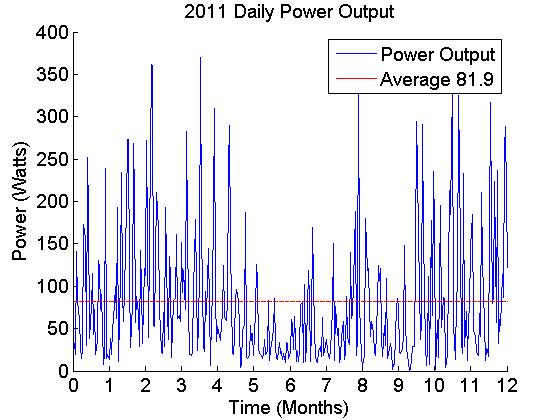
\includegraphics[width=\linewidth]{blum_figure4}
\caption{\textit{Hourly watt output}}
\label{fig:Hourly output in watts}
\end{figure}


\begin{figure}
\centering
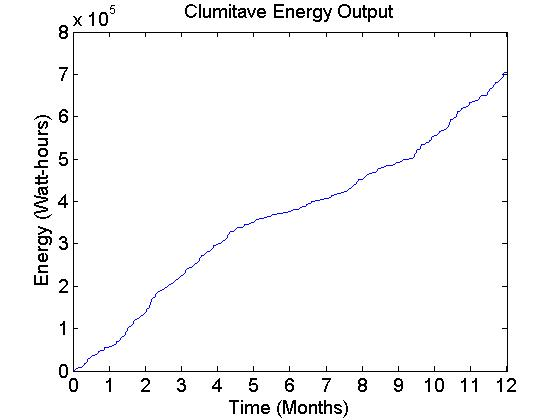
\includegraphics[width=\linewidth]{blum_figure5}
\caption{\textit{Cumulative power}}
\label{fig: Cumlative power}
\end{figure}

From the NOAA data and the wind turbine, we can determine the longest time there will be no output from the turbine. This is because the cut-in speed for this turbine is 3.2 meters per second. This will help to determine the battery size. 

\begin{table}
\centering
\begin{tabular}{|l|l|l|l|l|l|l|l|}\hline
Year & 2007 & 2008 & 2009 & 2010 & 2011 & 2012 &2013\\\hline
Hours & 175 & 263 & 219 & 243 & 103 & 664 & 110\\\hline
Days & 7.3 & 10.9 & 9.1 & 10.1 & 4.3 & 27.6& 4.5\\\hline
\end{tabular}
\caption{\textit{Time without power production}}
\label{tab:widgets}
\end{table}

		
\section{Battery Selection}
\indent The factors that were important in selection of a battery for energy storage were the size and specific battery chemistry. 
Each battery chemistry such as lead acid, nickel metal hydride or lithium ion, have certain advantages depending on the application. 
Most energy scavenging systems use lead acid as they allow for trickle charging. 
Lead acid batteries  however are larger and bulkier than others such as lithium batteries. 
For that reason, the battery chemistry proposed for this project was lithium polymer.
Other properties to take into account when selecting a battery are the energy density as well as the number of recharge cycles one can get out of the battery. 
Figure 3.13 is an illustration of mass and volume energy densities specific to the various battery chemistries. It is clear that lead acid and lithium polymer reside on opposite ends of the plot. 
\indent Lithium polymer batteries are exceptionally useful in applications that have space limitations such as remote operated vehicles. For this project, all of the hardware must fit inside of a case for weather proofing, making "LiPo" a reasonable selection for rechargeable battery. 
Another advantage to using lithium polymer is that they can be made into any shape or size. 
\indent Using the power budget listed above, which highlights the power consumption relative to each piece of the package, a battery was selected. To be conservative, the power budget was doubled, making the package a 7 watt system. It was determined that in a worst case scenario, the rechargeable battery must be capable of powering the package for a minimum of 3 days. After researching various capacities of batteries, two 12 AmpHour Lithium Ion batteries were purchased. The purchase of lithium ion over lithium polymer was due to misunderstanding, however testing was still carried out in order to generate discharge curves. In the future progress of this project, the design of a charge controller capable of accepting both solar and wind as well as being able to manage the charge of lithium polymer batteries must be implemented. In order to use battery chemistries such as lithium polymer/ion coupled with such a high power wind turbine, a charge controller is paramount. 

\begin{figure}
\centering
\includegraphics[width=\linewidth]{Battery_Chemistry}
\caption{\textit{Mass and Volume Energy Densities for Various Battery Chemistries}}
\label{fig:Battery_Chemistry}
\end{figure}

\chapter{Data Collection}
\label{ch:DataCollection}
	\section{Phase One Data Collection}
		\subsection{6g Tri-Axial Accelerometer Data}
			\input{Paul_DataCollection_6gTri-AxialAccelerometerData}
	\section{Phase Two Data Collection}
			\input{WESLEY_sixg}
			\input{WESLEY_cell}
			\input{WESLEY_battery}
			\input{WESLEY_solar}
			\input{WESLEY_wind}
		
\chapter{Data Analysis}
\label{ch:DataAnalysis}
	\section{Phase One Data Analysis}
		\subsection{Comparison of Preliminary Abaqus Model and Preliminary Data}
			\input{Paul_DataAnalysis__PhaseOne}
	\section{Phase Two Data Analysis}
		\subsection{Comparison of Developed Abaqus Model with Literature}
			\input{Paul_DataAnalysis_PhaseTwo_AbaqustoLit}
		
\chapter{Future Development}
\label{ch:FutureDevelopment}
	\section{Instrumentation}
		\subsection{Integration of Strain Gauge}
			\input{WILEY_Strain}
		\subsection{Wireless Transmission}
			\label{sec:XBeeFuture}
			\input{KIRBY_Future_Wireless}
		\subsection{GPS Time Synchronization}
			\input{IANNUCCI_TimeSync}
		\subsection{Package Assembly}
			\subsubsection{Fabrication of Printed Circuit Board}
				\input{KIRBY_Future_PCB}
			\subsubsection{Package Enclosure}
				\section{Package Enclosure}

When the components are tested and fully operational in laboratory conditions, they will need to be packaged into the casing. The following
characteristics need to be considered when determining which case is best suited for this application:

\begin{itemize}
\item {Quality} 
\item {Size/Orientation}
\item {Heat Dissipation} 
\item {Cost} 
\item {External Connectors}
\end{itemize}


When the package is mounted onto the Newport Bridge, it will be exposed to harsh weather conditions: wind, precipitation, extreme temperatures,
etc. Therefore, it is essential to utilize a case that can withstand these conditions. O-rings are necessary to prevent water from leaking into
the case through the seal of the lid. This water can easily damage the electrical components within the package. The case will also have to be able to
withstand possible extreme temperatures. If the case cannot withstand the possible cold temperatures it will be exposed to without cracking, water can
leak into the package and destroy the equipment. High temperatures can cause the case to melt/deform which may possibly affect the retrieved data. 

It will be important to choose a case that not only large enough that can house all of the equipment but also fits the equipment in a manner that it can
be neatly organized and arranged. This allows for a quicker and more efficient package assembly. This also allows for a quicker examination of the
set-up in case an error occurs. To account for this, the orientation of the case is important. For example, a top-loading bucket (such as the Pelican
1430 seen below) would not be practical because it would be very difficult to access the components once the package is assembled and mounted.  



Electrical devices are only operational within a specific temperature range where if the maximum or minimum temperatures are exceeded, the component may
not fully function or even fail completely. To determine if the SHM system will fail due to extreme temperatures, the temperature inside the case must
be calculated. The enclosed volume has two major sources of temperature flux: the external temperature and the work done by the system. The first step
will be to calculate the heat transferred from the electrical components using the equation:

\begin{equation}
q(eq) = P(eq)*K_1*K_2
\end{equation}

where $q(eq)$ is the heat transferred from electrical equipment in Watts (W), $P(eq)$ is the electrical power consumption (W), $K_1$ is the load
coefficient, and $K_2$ is the running time coefficient. This value will then be inserted into the 1-D heat transfer equation:

\begin{equation}
q=k*A*\frac{\Delta T}{dx}
\end{equation}

where $q$ is the heat due to the electrical components, $k$ is the thermal conductivity of the material, $A$ is the area of which heat is being transfered
through, $\Delta T$ is the change in temperature, and $dx$ is the thickness of material. This equation will need to be computed for the heat transfer
through each of the casing walls, as well as the corners of the case, then averaged using the equation: 

$$q_t = sqrt((q_x)^2+(q_y)^2+(q_z)^2+(q_c)^2)$$

where $q_c$ is the heat transfer through the corners of the case. The resulting value will then be used with the maximum expected temperatures based on
temperature history data, such as that provided by NOAA, to determine the maximum temperature at which the system will still operate. If the resulting
temperature is higher than the lowest maximum operating temperature out of all the components, the system may fail, and that case may not be the best
option. That same principal can be applied to when the system is not generating any heat with respect to the minimum expected external temperature and
highest minimum operational temperature of the components. Ideally, once the package is fully modeled, the heat transfer equation can be more
thoroughly and accurately calculated by accounting for the spatial orientation between the components and the interior walls of the case. However,
if the components are mounted in place via foam cutouts, the heat dissipation between the components and the foam must first be calculated, and then
the heat transfer between the foam and the interior walls will then be calculated.

\paragraph{External Connectors} 
Several external connectors will need to be installed on the case walls for the full functionality of the SHM system. These ports need to be waterproof
with tight seals to prevent water from entering the case or external connections. The waterproof connections will require secure mating mechanisms, such
as locking and screwing mechanisms shown in Figure \ref{fig:BowChicaWowWow}, to ensure that that the male ends will not become unplugged thus allowing
water to enter the connection and damage it. Each connector will also require a bulkhead cap to cover and protect against water damage if the
connector is not in use. These external connections are going to be implemented for a variety of sub-systems within the SHM package: energy
scavenging devices, BeagleBone Black, strain gauge, GPS, and XBee.
\begin{figure}[h]
\centering
\includegraphics[width=0.3\textwidth]{Wiley_MatingStyle.JPG}
\caption{\textit{Example Mating Mechanisms}}
\label{fig:BowChicaWowWow}
\end{figure}

Power connectors will be used to connect the wind turbine and solar panels to the package. These connectors must be rated for a high enough current to
match the power source. For example, since the wind turbine is rated up to 27A, the power connector should have a current rating that is similar enough
that there will not be damage done to the port due to the excess current. Each power connection will have a female port installed on the side of the
case and a corresponding male jack will need to be installed at the end of the power input. If multiple solar panels are utilized, either the power
inputs need to be put into parallel in one wire to input all the energy through one connection or a connector needs to be installed for as many panels
are used. 

A USB 2.0A port will be installed to access the BBB without having to open the package via a flash drive. This type of USB port was chosen to match the
same type of connection specified from the BBB data sheet. The connector gender of this port needs to be female to plug a USB chord to access the BBB,
such as the one seen in Figure \ref{fig:USB}. 
\begin{figure}[h]
\centering
\includegraphics[width=0.3\textwidth]{Wiley_USB2Aport.JPG}
\caption{\textit{USB 2.0A External Connector (LTWUA-20AMFM-SL7A) from Ampehnol LTW}}
\label{fig:USB}
\end{figure}

There are a few different types of connectors that can be used to attach the leads of the strain gauge to the package. Unlike the rest of the
connections, the strain gauge leads do not require a certain type of connection terminal. One option is to attach the leads to either a category 5 (CAT
5) or CAT5e shielded Ethernet cable and install an external connection for such a cable as seen in Figure \ref{fig:CAT5}. Category type cables are
designed for high signal integrity to achieve performance standards set by organizations \cite{gareis2003surfaced}. This type of cable will ensure that the signals are relayed to the ADC reliably. A shielded cable is desired to
ensure that the sensitive signal being sent from the strain gauge to the ADC does not get disturbed by noise. 
\begin{figure}[h]
\centering
\includegraphics[width=0.3\textwidth]{Wiley_CAT5EthernetConnection.JPG}
\caption{\textit{Shielded Ethernet External Connector (RJ45-5EWTP-QR-PCB) from Video Production Inc}}
\label{fig:CAT5}
\end{figure}

An alternative method is through the use of waterproof cable glands (see Figure \ref{fig:Cable Gland}. The leads would be attached to a cable, preferably
shielded, and fed through the gland which would then be sealed. The proper gland must be matched up to the outer diameter of the cable otherwise the
gland will not be water tight. These are advantageous because not only do individual cable glands work with a range of cable thicknesses, but different
gland diameter ranges can be found. 
\begin{figure}[ht]
\centering
\includegraphics[width=0.7\textwidth]{Wiley_CableGland.JPG}
\caption{\textit{Cable Gland (CB-GD-5000045) from AA Power Corp}}
\label{fig:Cable Gland}
\end{figure}


The GPS antenna attaches to the GPS via the use of a coaxial MCX connection. Two viable options for connecting the antenna are to implement a waterproof
MCX connector or a cable gland. Implementing a waterproof MCX connector on the package may be difficult because MCX connectors are very small as evident
by Figure \ref{fig:MCX}. If one of these connectors is able to implemented, it will be essential to choose the proper impedance level of the
connector. The other option is to implement a cable gland, such as the alternative option for the strain gauge above in Figure \ref{fig:Cable Gland},
to run a wire through the case wall between the antenna and the GPS. The antenna would then need to be fastened to the outside of the case or another
substrate to prevent it from freely swinging around. 
\begin{figure}[ht]
\centering
\includegraphics[width=0.7\textwidth]{Wiley_MCX.JPG}
\caption{\textit{MCX Jack-to-Jack Adapter (252171) from Aamphenol Connex with Size Reference}}
\label{fig:MCX}
\end{figure}


The final component that requires and external connector is the XBee.The XBee antenna attaches to the device itself via the use of an SMA connection. A
waterproof coaxial connector, like the one shown in Figure \ref{fig:SMA}, can be implemented as the external connector as well as a cable gland. 
Similarly to the MCX connector, the SMA connector is also small which may make utilizing one of these difficult. However, if a cable gland is used, the
antenna may need to be mounted to the case or other substrate to prevent it from freely swinging around as is the case with the GPS.
\begin{figure}[ht]
\centering
\includegraphics[width=0.7\textwidth]{Wiley_SMAconnector.JPG}
\caption{\textit{Waterproof SMA Bulkhead Connector (9153-7553-002) from Applied Engineering Products with Size Reference}}
\label{fig:SMA} 
\end{figure}



\paragraph {Case Selection} Attempts were made to try to obtain the actual thermal conductivity coefficients for different cases, but unfortunately proper
data was never able to be retrieved due to lack of information from retailers. Since the general material of the considered cases is known, an
estimation of the thermal conductivity coefficient was made because studies have been performed to determine $k$ values for different materials. 
However, continued efforts to obtain this information may supply data to more accurately calculate the heat transfer through the casing walls. The
thickness of each case will need to be considered for two reasons. The first reason is that the thickness of the case affects heat transfer. Thicker
cases will allow for less heat transfer through the casing walls. The other is that the thickness of the casing wall affects whether or not certain
external connectors can be implemented. If the case is too thick, many MCX and SMA connectors may not be able to be installed because the case may
be thicker than the connector is long. When comparing costs, it should be later noted of any accessories, whether they are necessary or
convenient, that can and will be purchased. For example, the Ultra-case 613 by UW Kinetics charges another \$6.99 for the required O-ring to
water proof an already expensive case, so this may not be the most suitable case for this application. For a look at the a comparison of nominal
characteristics of the cases that were considered, see \ref{sec:Appendix Case Comparison}.

\paragraph{Assembly Layout}
When the package is ready to be assembled, the interior layout of the components needs to be determined. A few factors will need to be considered. 
The first is the location of external connectors. As stated above, the thickness of the case will affect what type of connectors may need to used. 
An example of this is shown in Figure \ref{fig:Assembly} which is a potential 2-D assembly layout using a Pelican 1400 model case. 
If an SMA connector were to be utilized, it would need to be used on one of the shorter walls since they are thinner.  However, this SMA connector is barely longer than the case is thick and would not leave enough room to physically install it.  Therefore, a cable gland would need to be utilized as an external connector for a Pelican 1400 model case.  
It would not make to sense to install the connectors through the lid either because opening the case may place too much tension on the wires causing damage. 


\begin{figure}[h]
\centering
\includegraphics[width=1\textwidth]{Wiley_2DAssemblyLayout.jpg}
\caption{\textit{Potential Layout of a Pelican 1400 Model Case.
The red arrows depict a 12V power supply, the yellow arrows depict a 3.3V power supply, and the green arrows depict the transfer of communications.}}
\label{fig:Assembly}
\end{figure}

It will also be important to orient the breadboard in a manner that the accelerometer measures data in the intended direction as if it was mounted. 
Otherwise, it will need to be understood that the data measured on each axis during lab trials will not be measured along the same axes in the field and
will need to be accounted for while analyzing the data. 

			\subsubsection{Package Location}
				\input{MCINTOSH_PackageLocation}
	\section{FEM}
		\input{Paul_FutureDevelopments}
		
\chapter{Conclusion}
\label{ch:Collection}
	\input{Paul_Conclusion}
	
\bibliographystyle{plain}
\bibliography{./BIB_Files/McINTOSH_BIB,./BIB_Files/WILEY_BIB,./BIB_Files/KIRBY_BIB,./BIB_Files/IANNUCCI_BIB,./BIB_Files/WESLEY_BIB,./BIB_Files/BLUM_BIB,./BIB_Files/PAUL_BIB}

\appendix

\chapter{Sensor Package Schematics}
\label{app:Schematic}
\input{KIRBY_Schematics}

\chapter{Enclosure Options}
\label{app:CaseOptions}
\input{WILEY_CaseComp}

\chapter{Battery Log}
\label{app:batterylog}
\input{WESLEY_batterylog}
 

\end{document}
